\documentclass{article}
\usepackage{titlesec}
\usepackage{lipsum}
\usepackage{hyperref}
\usepackage{graphicx}
\usepackage{appendix}
\usepackage[left=1 in,right=1 in,top=1 in,bottom=1 in]{geometry}

% Remove the red boxes around links
\hypersetup{
    colorlinks=true,
    linkcolor=black, % You can change link colors to your preference
    citecolor=green, % You can change citation colors to your preference
    urlcolor=blue % You can change URL colors to your preference
}

\begin{document}
% Title Page
\begin{titlepage}
    \centering
    
\includegraphics[width=0.8\textwidth]{image.jpeg}\par % Adjust the width as needed
     \vspace{2cm}
    {\scshape\Large SOEN 6481: TAS REPORT \par}
    \vspace{1.5cm}
    {\scshape\Huge "Topic 58: How should I manage adoption of new technologies or processes in my projects?"\par}
    \vspace{1.5cm}
    {\large Advisor: Professor Pankaj Kamthan\par}
    \vspace{1.5cm}
    {\large By: Konark Shah (Student ID: 40232277)\par}
    \vspace{1cm}
    {\large \today\par}
\end{titlepage}



\tableofcontents

\newpage

\section{Abstract}
Even when there are compelling reasons to adopt new technologies or processes in projects, managing change is challenging. This report explores the factors to consider, such as the nature of the project and the experience of the team, when analyzing the costs and benefits of adopting new technologies or processes.

\section{Introduction}
In today's fast-changing tech landscape, it's crucial for companies to keep up with the competition by adopting and integrating new technologies into their existing products. Making the right decisions in this process is complex and can make or break a new product. To navigate this terrain successfully, one must consider a range of factors, including the nature of the ongoing project, the team's experience and skill set, communication strategies with stakeholders, and the pivotal step of securing approval from top management. This thesis seeks to unravel the complexities surrounding this crucial decision-making process, offering insights into the managerial intricacies involved in the successful adoption of new technologies or processes within projects.

\subsection{Motivation}
This thesis is motivated by a keen interest in unraveling the complexities of adopting new technology and procedures. Recognizing that understanding this complexity is not just beneficial but essential for successful project navigation, the thesis aims to shed light on practical approaches for managing the adoption of new technologies. It aspires to offer valuable insights for project managers, helping them strike a delicate balance between innovation and seamless project execution.

\subsection{Problem Statement}
The fundamental issue addressed in this paper is the successful management of new technology or process adoption within project environments. The complexity stems from the opposition encountered during major changes, the uncertainties around cost and benefit projections, and the requirement for a proactive strategy to obtain buy-in from contributors and stakeholders. Prudent decision-making in this setting necessitates a thorough awareness of the issues at hand, as well as the creation of appropriate mitigation methods.

\subsection{Objectives}

The objectives of this investigation are to:
\begin{itemize}
  \item Evaluate the impact of project nature and team experience on technology and process adoption.
  \item Analyze the costs of staying with the current methods and transitioning to new technologies or processes.
  \item Determine the monetary benefits of adopting new technologies or processes.
  \item Identify effective techniques for overcoming internal organizational resistance to the adoption of new technologies.
  \item Recognize and analyze the limitations of various solutions and explore their future scope.
\end{itemize}

The purpose of this research is to provide significant insights to project leaders, managers, and stakeholders, equipping them with information and techniques to efficiently negotiate the challenging terrain of technology adoption in project environments. This research aims to address the difficulties and uncertainties inherent in the adoption of new technologies or processes within project contexts by conducting a thorough examination of the aforementioned factors.

\section{Background Material}

The adoption and integration of new technology pose a managerial challenge with a substantial impact on overall corporate success. In this section, we will delve into the fundamentals, examining the nature of the project change, identifying various factors affected, essential mechanisms for the integration process, and outlining specific conditions that guide their effective utilization. This expertise is particularly valuable for managers overseeing technology integration, offering practical advice on navigating the process within their specific organizational contexts.

\subsection{Nature of the project change and their Impact}

Understanding a project before embracing change involves considering various factors. The primary factor is the organization's level of prior experience with technology integration, commonly referred to as technological maturity. The second factor revolves around assessing the extent to which the new technology contributes to product advancement. This evaluation involves determining whether the technology enhances the existing product's functionality beyond its original scope, thereby generating a strategic advantage. Alternatively, it considers scenarios where the new technology serves as an additional support function without altering the fundamental features of the core mechanical product [1].

\begin{figure}[h]
    \centering
    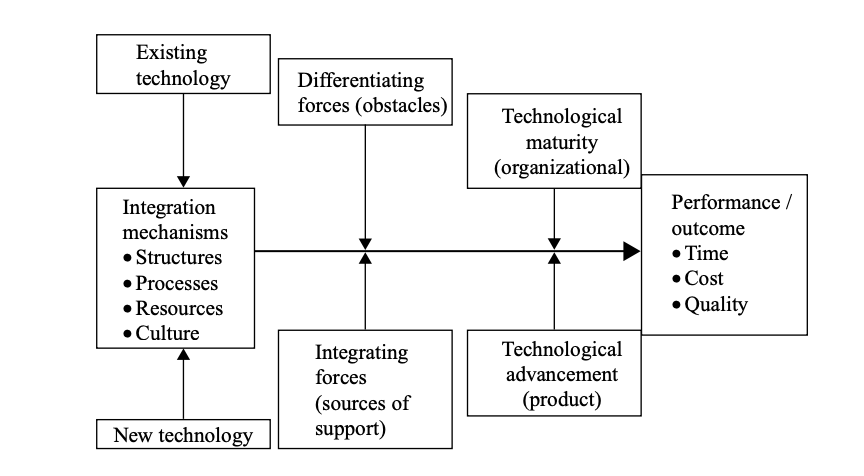
\includegraphics[width=0.8\textwidth]{Figure1.png}
    \caption{Conceptual model of the project change with implications and impact [1].}
    \label{fig:conceptual-model}
\end{figure}

\noindent The model in Figure 1 illustrates various things involved in during the project change and their impacts. Initially understanding the existing technology and the new to-be-adopted technology results in changes to the structures, processes, resources, and culture of the organization. Further into the picture are obstacles (differentiating forces) and sources of support (integrating forces) that influence the process. Finally, understanding the technological maturity of the current product/process and the advancement done to it, streamlining the analysis of their impacts, and taking deliberate steps based on this understanding as a project manager leads to favorable outcomes, benefiting the organization.

 
\subsection{Role of team experience in technology/process adoption}
The seamless adoption of technology within any project is intricately linked to the collaborative efforts of the involved team. The team's collective motivation, combined with their prior knowledge and skill sets, significantly shapes the trajectory of adoption, creating an environment conducive to successful integration. However, without proper attention, challenges such as resistance to change, gaps in knowledge, a resistant mindset, and a lack of collaboration can impede the technology/process adoption process. As rightly stated, "People's commitment to change increases the chance of successful transformation and decreases the cost of change. It is the most powerful catalyst for changing approach" [2].

\section{Methods \& Methodology}

\subsection{Analyzing costs and benefits}
When major changes are part of a project, planning conservatively is vital. This includes reassessing team skills, considering learning curve issues, and preparing for potential risks and unknowns.
\subsection{Estimation Process}
Securing buy-in from project stakeholders is crucial for successful adoption. This involves building support through facts, figures, and effective communication.
\subsection{Verification of Estimates}
Securing buy-in from project stakeholders is crucial for successful adoption. This involves building support through facts, figures, and effective communication.
\subsection{Planning for change}
Securing buy-in from project stakeholders is crucial for successful adoption. This involves building support through facts, figures, and effective communication.
\subsection{Securing Buy-In}
Securing buy-in from project stakeholders is crucial for successful adoption. This involves building support through facts, figures, and effective communication.
\subsection{Overcoming Resistance}
Securing buy-in from project stakeholders is crucial for successful adoption. This involves building support through facts, figures, and effective communication.



\section{Results Obtained}
\subsection{Under What Conditions}
The conditions that favor successful adoption of new technologies or processes are influenced by project nature and team experience.
\subsection{Constraints}
Constraints may arise due to resistance to change, unrealistic cost estimates, or challenges in securing buy-in.
\subsection{Quality Assessment}
The quality of technology and process adoption can vary depending on the level of planning, conservative estimation, and securing buy-in.

\section{Conclusions and Future Works}
\subsection{Limitations to Solution}
While the proposed approach can be effective, it may not work well in projects with deeply entrenched resistance to change or in cases where accurate cost estimation is challenging.
\subsection{Suggested Improvements}
To improve the management of technology and process adoption in projects, it is recommended to:
\begin{itemize}
  \item Enhance project planning and estimation.
  \item Develop effective strategies for securing buy-in.
\end{itemize}
\subsection{Applications in Real World}
The solutions presented in this report can be applied in various real-world scenarios, including project management, organizational change, and technology adoption.
\subsection{Conclusion}
In conclusion, managing the adoption of new technologies and processes in projects requires careful planning, estimation, and communication. Success is contingent on understanding project nature and team experience, as well as securing buy-in from stakeholders.

\section{References}
\begin{enumerate}
  \item Karlsson, C., Taylor, M., \& Taylor, A. (2010). Integrating new technology in established organizations: A mapping of integration mechanisms. \textit{International Journal of Operations \& Production Management, 30}(7), 672--699. Emerald Group Publishing Limited.
  
  \item Gandomani, T. J., Zulzalil, H., Ghani, A. A., Sultan, A. B. M., \& Sharif, K. Y. (2014). How human aspects impress Agile software development transition and adoption. \textit{International Journal of Software Engineering and Its Applications, 8}(1), 129--148.
  
  % Add more references as needed
\end{enumerate}



\section{Acknowledgements}
I would like to acknowledge the invaluable contributions of ChatGPT, Perplexity, and my favorite YouTube channel for their insights and inspiration. And also references of journal from Google Scholar.

\end{document}